\begin{surferIntroPage}{Einfache Singularitäten}{simplesing_A1pm}{Einfache Singularitäten}
 Eine Fläche heißt \emph{nicht-singulär} oder \emph{glatt}, wenn sie,
    anschaulich gesagt, 
    keine spitzen Stellen (\emph{Singularitäten} genannt) hat, z.B.\ eine Kugel, 
    ein Torus (s.\ Abb.). 
    \begin{center}
      \vspace{-0.2cm}
      \begin{tabular}{@{}c@{}c@{}c@{\quad}c@{}c@{}c@{}c@{}}
        \begin{tabular}{@{}c@{}}
          glatt:
        \end{tabular}
        &
        \begin{tabular}{@{}c@{}}
          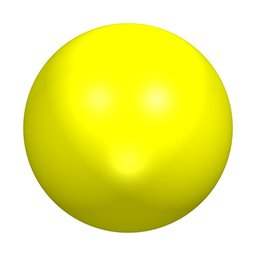
\includegraphics[width=1.1cm]{../../common/images/kugel}
        \end{tabular}
        &
        \begin{tabular}{@{}c@{}}
          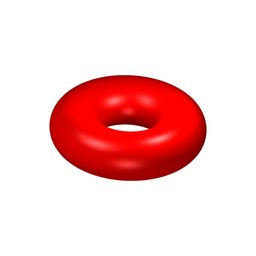
\includegraphics[width=1.1cm]{../../common/images/torus}
        \end{tabular}
        &
        \begin{tabular}{@{}c@{}}
          singulär:
        \end{tabular}
        &
        \begin{tabular}{c@{}@{}}
          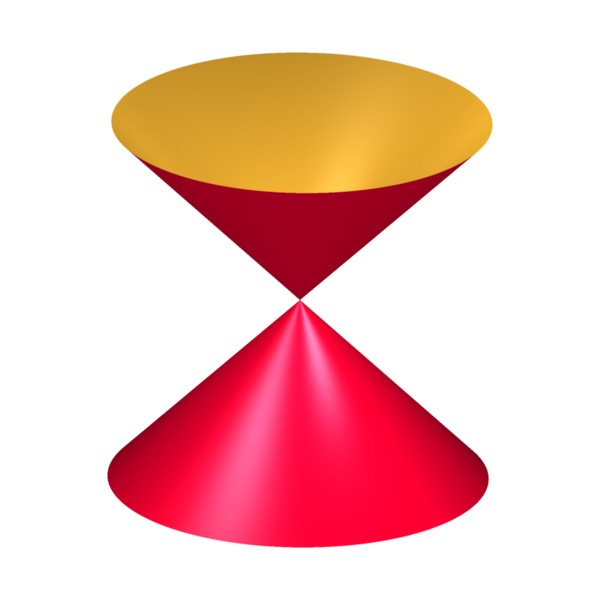
\includegraphics[width=1.1cm]{../../common/images/kegel}
        \end{tabular}
        &
        \begin{tabular}{c@{}@{}}
          
\includegraphics[width=1.1cm]{../../common/images/A2pm}
        \end{tabular}
        &
        \begin{tabular}{c@{}@{}}
          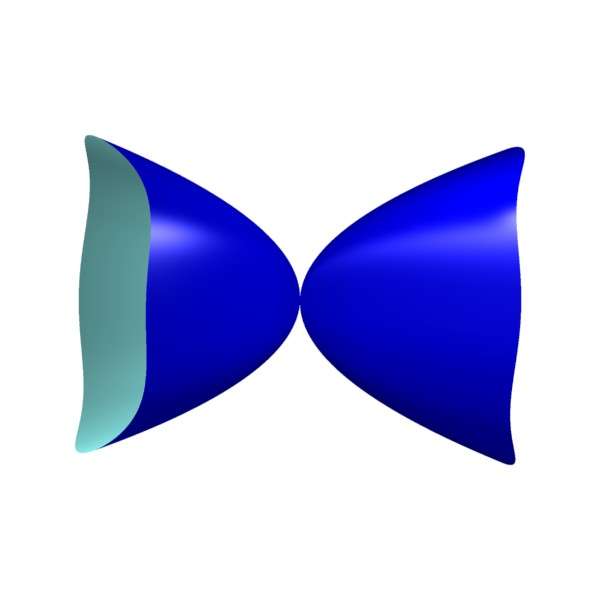
\includegraphics[width=1.1cm]{../../common/images/A3pm_0}
        \end{tabular}
      \end{tabular}
    \end{center}
    \vspace{-0.2cm}
    Die sogenannten \emph{ADE-Singularitäten} sind die einfachsten
    Singularitäten.   
    Beispiele sind Singularitäten vom Typ $A_k^{\pm\pm}$ mit Gleichung
    $x^{k+1}\pm y^2\pm z^2=0$. 
    Im obigen Bild, ganz rechts: 
    $A_3^{+-}$, daneben $A_2^{+-}$ und $A_1^{+-}$ (auch \emph{Doppelkegel}
    genannt). 

    Die ADE-Singularitäten haben ganz erstaunliche Beziehungen 
    zu unzähligen anderen Gebieten der Mathematik, Physik sowie belebter
    und unbelebter Natur, die bis heute nicht völlig verstanden sind.

    Jede $A_k$-Singularität lässt sich in $\lfloor\frac{k+1}{2}\rfloor$
    $A_1$-Singularitäten deformieren; für $A_3^{+-}$ ergeben
    sich zwei $A_1^{+-}$-en (s.\ Abb.\ links): 
%    \dontshow{
    % 
    \begin{center}
      \vspace{-0.2cm}
      \begin{tabular}{@{}c@{\quad}c@{}c@{\qquad\quad}c@{\quad}c@{\quad}c@{}}
        \begin{tabular}{@{}c@{}}
          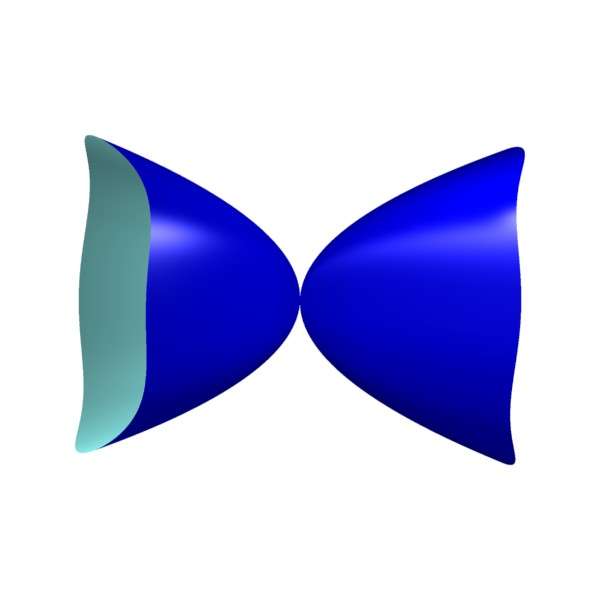
\includegraphics[width=1.2cm]{../../common/images/A3pm_0}
        \end{tabular}
        &
        \begin{tabular}{@{}c@{}}
          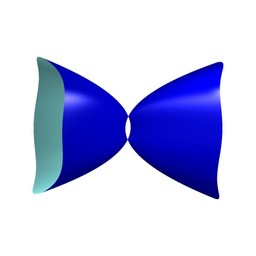
\includegraphics[width=1.2cm]{../../common/images/A3pm_1}
        \end{tabular}
        &
        \begin{tabular}{@{}c@{}}
          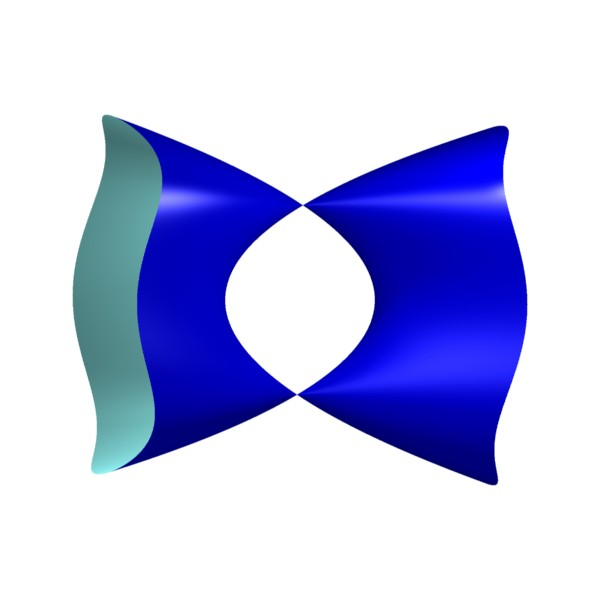
\includegraphics[width=1.2cm]{../../common/images/A3pm_2}
        \end{tabular}
        &
        \begin{tabular}{@{}c@{}}
          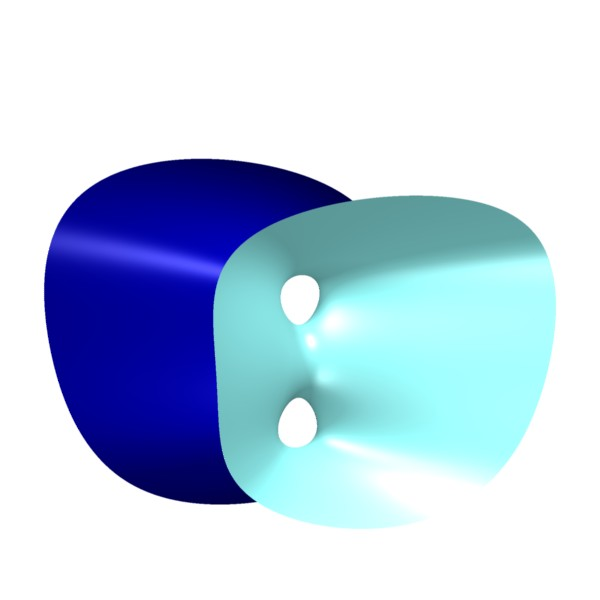
\includegraphics[width=1.2cm]{../../common/images/A3pm_vz_2}
        \end{tabular}
        &
        \begin{tabular}{@{}c@{}}
          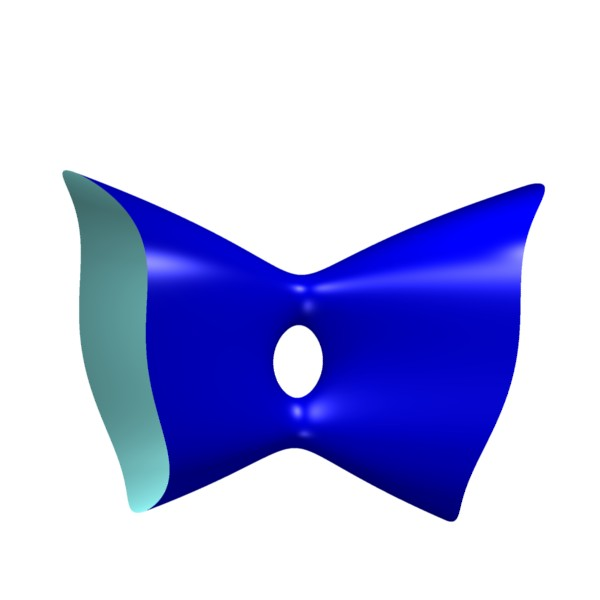
\includegraphics[width=1.2cm]{../../common/images/A3pm_vz_1}
        \end{tabular}
        &
        \begin{tabular}{@{}c@{}}
          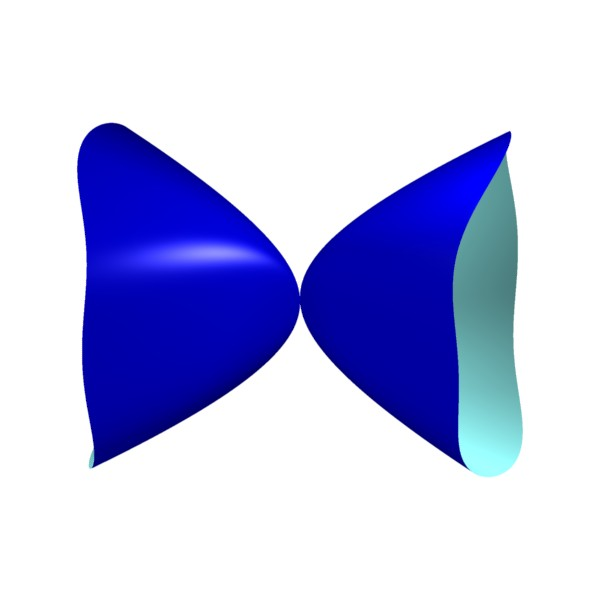
\includegraphics[width=1.2cm]{../../common/images/A3pm_vz_0}
        \end{tabular}
      \end{tabular}
      \\
      \begin{tabular}{@{}c@{\qquad\qquad}c@{}}
          $A_3 \qquad\quad \rightarrow \qquad 2 A_1$
          &
          $2$ Zykel $+$ $1$ Zykel \ $\rightarrow \ A_3$
        \end{tabular}
    \end{center}
%    }
    \vspace*{-0.2cm}
    Der Index $k$ der $A_k$-Singularitäten ist die sog.\ \emph{Milnor-Zahl} der
    Singularität; dies ist die Anzahl der sog.\ \emph{verschwindenden
    Zykel}, d.h.\ der ``Durchgänge'', die verschwinden, wenn man sie
    zur Singularität zusammenzieht (s.\ Abb.\ rechts).  
\end{surferIntroPage}
